\documentclass{article}
\usepackage{amsmath,amssymb}
\usepackage{tikz}
\usetikzlibrary{shapes,arrows,positioning}
% Language setting
% Replace `english' with e.g. `spanish' to change the document language
\usepackage[english]{babel}
\nocite{*}


% Set page size and margins
% Replace `letterpaper' with `a4paper' for UK/EU standard size
\usepackage[letterpaper,top=2cm,bottom=2cm,left=3cm,right=3cm,marginparwidth=1.75cm]{geometry}

% Useful packages
\usepackage{amsmath}
\usepackage{graphicx}
\usepackage{array}
\usepackage[colorlinks=true, allcolors=blue]{hyperref}
\title{%
Teaching Assignment\\
\vspace{0.5cm}
  \textbf{Fuzzy Relations}\\
  \large ( Propreties, Operations, and $\alpha$-cut)\\
  \vspace{0.8cm}
  Course : BITS F343 Fuzzy Logic and Applications\\
  \vspace{0.1cm}
  Instructor: Dr. Chandra Shekhar 
  \vspace{0.5cm}
  }
\author{
  Anish Kulkarni\\
  \texttt{2020A7PS0975P}
  \and
  P V S Tarak Shree Vallabha\\
  \texttt{2020A7PS1513P}
  \and
  Dr. Chandra Shekhar\\
  \texttt{csbits.fuzzy@gmail.com}
\vspace{0.6cm}
}

\date{December 10, 2022}
\begin{document}
\maketitle

\begin{abstract}
The concept of fuzzy relations is developed from the concepts of crisp relations and fuzzy sets. Various representations and operations associated with fuzzy relations are discussed along with their examples. Properties of fuzzy relations are defined. The document also includes discussion about the $\alpha$-cut of fuzzy relations. Finally, the document ends with a few exercises related to the above mentioned topics. 
\end{abstract}

\section{Introduction}

Just as fuzzy sets can be thought of as an extension of crisp sets, relations between crisp sets can be extended to relations between fuzzy sets. The document begins with an introduction of crisp relations and fuzzy relations. Subsequently, the concept of alpha cut for fuzzy relations will be introduced and finally we will see various operations related to fuzzy sets.

\section{Crisp Relations}
The word ‘relation’ means a connection between two entities. For example, consider two entities “courses” and “rooms”. A relation between the two could be defined specifying the room in which a course is conducted. Formally, a crisp relation(R) is defined on crisp sets $S_1, S_2, S_3.....S_n$ as a subset of the Cartesian product of all the sets.
\[R\subseteq S_1 \times S_2 \times...\times S_n \quad \textrm{where} \quad n>=2\]or,
\[R = \{(x_1,x_2,x_3,...,x_n) \mid x_1\in S_1 , x_2\in S_2,...,x_n\in S_n,\quad n>=2 \} \]$\textbf{Example 1}$\newline Consider the example mentioned above. Let
\[courses=\{"FLA","DSA","OS","DBS"\}\quad and\]
\[rooms=\{"1234","5102","5105","6151"\}\quad \]

The relation R : $courses \times rooms \rightarrow \{0,1\}$ can be specified as 
\[R = \{("DSA","5102"),("OS","5105"),("FLA","6151"),("DBS","5102"),("DSA","1234")\} \]
Depending on the value of n, relations can be categorized into different types. R is defined on two sets and hence it is called as a Binary Relation.\newline
With respect to any crisp relation we can define a function known as the characteristic function ($\chi$). It maps the Cartesian product of n sets to the set {0,1}. Let A and B be two crisp sets related by a relation R.

\begin{equation}
\chi_{A \times B}(a,b)=
    \begin{cases}
        1 & \text{if } x \in A\times B\\
        0 & otherwise\\
    \end{cases}
\end{equation}



\section{Fuzzy Relations}

Essentially all crisp relations are sets which have tuples as its members. Each tuple of a crisp relation has a strength associated with it. This is defined by the Characteristic Function and it can take only two values (0 or 1). Fuzzy relations are relations that are defined on Fuzzy sets. They have characteristic function values ranging from [0,1]. In this case we call the characteristic function as the membership function ($\mu$) . Fuzzy relations are subsets of Cartesian products of Fuzzy sets.\newline
For simplicity consider  fuzzy sets $\Tilde{R}$,$\tilde{A}$ and $\tilde{B}$ where,
\begin{equation}
\Tilde{R}=\{(a,b),\mu(a,b)\mid (a,b)\in A\times B\}
\end{equation}
The above fuzzy set $\Tilde{R}$ will be a fuzzy relation on $\Tilde{A} \times \Tilde{B} \hspace{0.1cm} only \hspace{0.1cm}if\hspace{0.1cm}  it\hspace{0.1cm}  is\hspace{0.1cm}  a \hspace{0.1cm} subset \hspace{0.1cm}  of\hspace{0.1cm}  \Tilde{A}\times\Tilde{B}, i.e.$ 
\[\mu(a,b) \leq min\{\mu(a),\mu(b)\}\quad where\quad a\in\Tilde{A} , \hspace{0.1cm} b\in \Tilde{B}\quad and\quad (a,b)\in\Tilde{R}\]
$\textbf{Example 2}$\newline Consider a set A
\[A=\{a,b,c,d\}\] We can define a fuzzy relation $\Tilde{R}\hspace{0.1cm}on \hspace{0.1cm} A\times A$ given by
\[\Tilde{R} = \{((a,a),1),((b,b),0.5),((c,c),1),((d,d),0.5),((a,b),0.2),((b,c),0.3),((c,d),0.4),((d,a),0.5)\} \]


\subsection{Representation of Fuzzy Relations}
\subsubsection{Like Fuzzy Sets}
1. Defined in equation(2) \newline\newline
2. $\Tilde{R}(a,b)=\Bigl\{ \frac{\mu_{\Tilde{R}}(a,b)}{(a,b)}\hspace{0.1cm}\mid\hspace{0.1cm} (a,b)\in A\times B \Bigl\}$
\subsubsection{Tabular form}
Let $\Tilde{R}$ be a ternary fuzzy relation defined on $\Tilde{A}\times\Tilde{B}\times\Tilde{C},$ where $\Tilde{A}=\{(a1,1),(a2,0.9)\} , \Tilde{B}=\{(b1,1),(b2,0.8)\},\Tilde{C}=\{(c1,0.9),(c2,0.8)\} $
\begin{center}
$\Tilde{R}\quad = \quad$
\begin{tabular}{ | m{1cm} | m{1cm}| m{1cm} | } 
  \hline
  c1& b1 & b2 \\ 
  \hline
  a1  & 0.5 & 0.4 \\ 
  \hline
  a2 & 0.1 & 0 \\ 
  \hline
\end{tabular}
\quad
\begin{tabular}{ | m{1cm} | m{1cm}| m{1cm} | } 
  \hline
  c2& b1 & b2 \\ 
  \hline
  a1  & 0.6 & 0.3 \\ 
  \hline
  a2 & 0 & 0 \\ 
  \hline
\end{tabular}
\end{center}
\subsubsection{Function form}
Let $\Tilde{R}$ be defined on $\Tilde{A}\times\Tilde{B}$ where
\[\mu_{\Tilde{R}}(a,b)=f(a,b)\quad;f \hspace{0.1cm} is \hspace{0.1cm} some \hspace{0.1cm}function\]
For example, $f=e^{-(a-b)^2}$ .
\subsubsection{Graph}
Consider $\Tilde{R}$ defined on $\Tilde{A}\times\Tilde{B}$. $\Tilde{R}$ can also be represented with a Graph G(v,e).\newline
Let v be any vertex and e($v_i,v_j$) be any edge of the graph from $v_i$ to $v_j$ such that e($v_i,v_j$) exists if $(v_i,v_j)\in \Tilde{R}$ and $v_i\in {\Tilde{A}}, v_j \in {\Tilde{B}}$. Example 2 can be represented in the following way:\newline\newline
\begin{center}
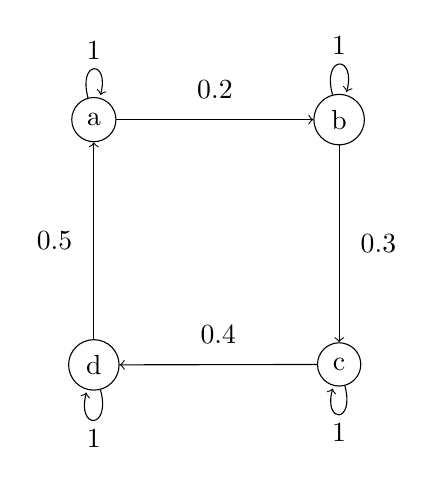
\begin{tikzpicture}[node distance=2.5cm]
\node[circle,draw](a){a};
\node[circle,draw](b)[right=of a]{b};
\node[circle,draw](c)[below=of b]{c};
\node[circle,draw](d)[below=of a]{d};
\path(a)edge[loop above]node{1}(a);
\path(b)edge[loop above]node{1}(b);
\path(c)edge[loop below]node{1}(c); 
\path(d)edge[loop below]node{1}(d);
\draw[->](a)--node[above=0.15cm]{0.2}(b);
\draw[->](b)--node[right=0.15cm]{0.3}(c);
\draw[->](c)--node[above=0.15cm]{0.4}(d);
\draw[->](d)--node[left=0.15cm]{0.5}(a);
\end{tikzpicture}
\end{center}
Here since the Universe is $\Tilde{A}\times\Tilde{A}$ the only nodes present in the graph will $\in$ \{a,b,c,d\}

\section{Operations on Fuzzy Relations}
We know that a Fuzzy Relation is also a type of Fuzzy Set. Hence, we can apply operations to this set. Assume $\Tilde{R}\in\Tilde{A}\times\Tilde{B}$ and $\Tilde{S}\in\Tilde{A}\times\Tilde{B}$. Here $\Tilde{R}$ and $\Tilde{S}$ are fuzzy relations defined on the Universe $\Tilde{R}\in\Tilde{A}\times\Tilde{B}$.

\subsection{Union}
The membership function for union of above two fuzzy relations is defined as
\begin{equation}
\mu_{\Tilde{R}\cup\Tilde{S}}(x,y)=max(\mu_{\Tilde{R}}(x,y),\mu_{\Tilde{S}}(x,y))\quad  ;\quad (x,y)\in {X}\times{Y} 
\end{equation}
$\textbf{Example 3}$\newline
\begin{center}
\def\arraystretch{1.4}%
\begin{tabular}{ | m{1cm} | m{1cm}| m{1cm} | } 
  \hline
  $\Tilde{R}$& b1 & b2 \\ 
  \hline
  a1  & 0.5 & 0.4 \\ 
  \hline
  a2 & 0.1 & 0 \\ 
  \hline
\end{tabular}
\quad
\def\arraystretch{1.4}%
\begin{tabular}{ | m{1cm} | m{1cm}| m{1cm} | } 
  \hline
  $\Tilde{S}$& b1 & b2 \\ 
  \hline
  a1  & 0.6 & 0.3 \\ 
  \hline
  a2 & 0 & 0 \\ 
  \hline
\end{tabular}
\end{center}
\begin{center}
\def\arraystretch{1.4}%
\begin{tabular}{ | m{1cm} | m{1cm}| m{1cm} | } 
  \hline
  $\Tilde{R}\cup\Tilde{S}$& b1 & b2 \\ 
  \hline
  a1  & 0.6 & 0.4 \\ 
  \hline
  a2 & 0.1 & 0 \\ 
  \hline
\end{tabular}
\end{center}
\subsection{Intersection}
The membership function for intersection of above two fuzzy relations is defined as
\begin{equation}
\mu_{\Tilde{R}\cap\Tilde{S}}(x,y)=min(\mu_{\Tilde{R}}(x,y),\mu_{\Tilde{S}}(x,y)) \quad  ;\quad (x,y)\in\ X\times Y    
\end{equation}
$\textbf{Example 4}$\newline
\begin{center}
\def\arraystretch{1.4}%
\begin{tabular}{ | m{1cm} | m{1cm}| m{1cm} |m{1cm} | } 
  \hline
  $\Tilde{R}$& b1 & b2 & b3 \\ 
  \hline
  a1  & 0.5 & 0.4 & 0.6 \\ 
  \hline
  a2 & 0.1 & 0 & 1 \\ 
  \hline
\end{tabular}
\quad
\def\arraystretch{1.4}%
\begin{tabular}{ | m{1cm} | m{1cm}| m{1cm} | m{1cm} |} 
  \hline
  $\Tilde{S}$& b1 & b2 & b3 \\ 
  \hline
  a1  & 0.6 & 0.3 & 0.7 \\ 
  \hline
  a2 & 0 & 0 & 0.2 \\ 
  \hline
\end{tabular}
\end{center}
\begin{center}
\def\arraystretch{1.4}%
\begin{tabular}{ | m{1cm} | m{1cm}| m{1cm} |m{1cm} | } 
  \hline
  $\Tilde{R}\cap\Tilde{S}$& b1 & b2 & b3\\ 
  \hline
  a1  & 0.5 & 0.3 & 0.6 \\ 
  \hline
  a2 & 0 & 0 & 0.2 \\ 
  \hline
\end{tabular}
\end{center}
\subsection{Complement}
The membership function for complement of any one of the above fuzzy relations is defined as
\begin{equation}
\mu_{\Tilde{R}^c}(x,y)=1-\mu_{\Tilde{R}}(x,y)\quad  ;\quad (x,y)\in\ X\times Y  
\end{equation}
$\textbf{Example 5}$\newline
\begin{center}
\def\arraystretch{1.4}%
\begin{tabular}{ | m{1cm} | m{1cm}| m{1cm} | m{1cm} |} 
  \hline
  $\Tilde{R}$& b1 & b2 &b3 \\ 
  \hline
  a1  & 0.5 & 0.4 & 0.6 \\ 
  \hline
  a2 & 0.1 & 0 & 1 \\ 
  \hline
\end{tabular}
\quad
\def\arraystretch{1.4}%
\begin{tabular}{ | m{1cm} | m{1cm}| m{1cm} |m{1cm} | } 
  \hline
  $\Tilde{R}^c$& b1 & b2 & b3 \\ 
  \hline
  a1  & 0.5 & 0.6 & 0.4 \\ 
  \hline
  a2 & 0.9 & 1 & 0 \\ 
  \hline
\end{tabular}
\end{center}
\subsection{Inverse}
The membership of the inverse of a fuzzy relation is defined by
\begin{equation}
\mu^{-1}_{\Tilde{R}}(y,x)=\mu_{\Tilde{R}}(x,y)\quad  ;\quad (x,y)\in\ X\times Y
\end{equation}
$\textbf{Example 6}$\newline
\begin{center}
\def\arraystretch{1.4}%
\begin{tabular}{ | m{1cm} | m{1cm}| m{1cm} | } 
  \hline
  $\Tilde{R}$& b1 & b2 \\ 
  \hline
  a1  & 0.5 & 0.4 \\ 
  \hline
  a2 & 0.1 & 0 \\ 
  \hline
\end{tabular}
\quad
\def\arraystretch{1.4}%
\begin{tabular}{ | m{1cm} | m{1cm}| m{1cm} | } 
  \hline
  $\Tilde{R}^{-1}$& b1 & b2 \\ 
  \hline
  a1  & 0.5 & 0.1 \\ 
  \hline
  a2 & 0.4 & 1 \\ 
  \hline
\end{tabular}
\end{center}
\subsection{Containment}
$\Tilde{R}$ is said to be contained in $\Tilde{S}$ if $\Tilde{R} \subseteq\Tilde{S}$.
\[\mu_{\Tilde{R}}(x,y)\leq\mu_{\Tilde{s}}(x,y)\quad\forall (x,y)\in\ X\times Y\]
\subsection{Composition}
The composition operation helps in combining fuzzy relations defined over different universes. This operation basically allows us to combine two or more relations into one. There are multiple ways to perform composition, one of which is using the min-max operation.\newline
\begin{equation}
    \mu_{\Tilde{R}\circ\Tilde{S}}(a,c)=\mathop{max}_{\forall b\in B}\{{min\{\mu_{\Tilde{R}}(a,b),\mu_{\Tilde{S}}(b,c)\}}\hspace{0.1cm} :\hspace{0.1cm} \Tilde{R} \in \Tilde{A}\times\Tilde{B},\hspace{0.1cm}\Tilde{S} \in \Tilde{B}\times\Tilde{C} 
\end{equation}
$\textbf{Example 7}$\newline\newline
Consider two fuzzy sets,one of which gives a relationship between the ripeness of a fruit and its color. The second fuzzy relation defines the relation between the taste and color of a fruit. After the composition of the two relations we get a new relation which defines the strength of association between the color of a fruit and its taste. \newline\newline
\begin{center}
\def\arraystretch{1.4}%
\begin{tabular}{ | m{1cm} | m{1cm}| m{1cm} | m{1cm}| } 
  \hline
  $\Tilde{R}$ & Unripe & Half-mature & Mature \\ 
  \hline
  Green & 1 & 0.2 & 0 \\ 
  \hline
  Yellow & 0.3 & 1 & 0.4\\ 
  \hline
  Red & 0 & 0.2 & 1 \\ 
  \hline
\end{tabular}
\quad
    \def\arraystretch{1.4}%
\begin{tabular}{ | m{1cm} | m{1cm}| m{1.4cm} | m{1cm}| } 
  \hline
  $\Tilde{S}$ & Sour & Tasteless & Sweet \\ 
  \hline
  Unripe & 1 & 0.2 & 0 \\ 
  \hline
  Half-mature & 0.7 & 1 & 0.3\\ 
  \hline
  Mature & 0 & 0.7 & 1 \\ 
  \hline
\end{tabular}
\end{center}
\begin{center}
    \def\arraystretch{1.4}%
\begin{tabular}{ | m{1cm} | m{1cm}| m{1.4cm} | m{1cm}| } 
  \hline
  $\Tilde{R}\circ\Tilde{S}$ & Sour & Tasteless & Sweet \\ 
  \hline
  Green & 1 & 0.2 & 0 \\ 
  \hline
  Yellow & 0.7 & 1 & 0.3\\ 
  \hline
  Red & 0 & 0.7 & 1 \\ 
  \hline
\end{tabular}
\end{center}
\subsection{Algebraic Product}
$\Tilde{R}$ and $\Tilde{S}$ are fuzzy relations on the product space X $\times$ Y. The membership function for the algebraic product of the two relations is given as :
\[\mu_{\Tilde{R}\stackrel{\wedge}{\times}\Tilde{S}}(x,y)=\mu_{\Tilde{R}}(x,y)\times\mu_{\Tilde{S}}(x,y)\quad;\quad \forall (x,y)\in X\times Y\]
$\textbf{Example 8}$\newline
\begin{center}
\def\arraystretch{1.4}%
\begin{tabular}{ | m{1cm} | m{1cm}| m{1cm} | } 
  \hline
  $\Tilde{R}$& b1 & b2 \\ 
  \hline
  a1  & 0.5 & 0.4 \\ 
  \hline
  a2 & 0.1 & 0 \\ 
  \hline
\end{tabular}
\quad
\def\arraystretch{1.4}%
\begin{tabular}{ | m{1cm} | m{1cm}| m{1cm} | } 
  \hline
  $\Tilde{S}$& b1 & b2 \\ 
  \hline
  a1  & 0.6 & 0.3 \\ 
  \hline
  a2 & 0.2 & 0 \\ 
  \hline
\end{tabular}
\end{center}
\begin{center}
\def\arraystretch{1.4}%
\begin{tabular}{ | m{1cm} | m{1cm}| m{1cm} | } 
  \hline
  $\Tilde{R}\stackrel{\wedge}{\times}\Tilde{S}$& b1 & b2 \\ 
  \hline
  a1  & 0.3 & 0.12 \\ 
  \hline
  a2 & 0.02 & 0 \\ 
  \hline
\end{tabular}
\end{center}

\section{Properties of Fuzzy Relations}
Let $\Tilde{R}$ , $\Tilde{S}$ , $\Tilde{T}$ , be fuzzy relations defined on the product space X$\times$ Y. They hold the following properties :\newline
\subsection{Commutativity}
\begin{equation}
    \Tilde{R}\cup\Tilde{S}=\Tilde{S}\cup\Tilde{R}
\end{equation}
\begin{equation}
    \Tilde{R}\cap\Tilde{S}=\Tilde{S}\cap\Tilde{R}
\end{equation}
\subsection{Associativity}
\begin{equation}
    \Tilde{R}\cup(\Tilde{S}\cup\Tilde{R})=(\Tilde{R}\cup\Tilde{S})\cup\Tilde{R}
\end{equation}
\begin{equation}
    \Tilde{R}\cap(\Tilde{S}\cap\Tilde{R})=(\Tilde{R}\cap\Tilde{S})\cap\Tilde{R}
\end{equation}
\subsection{Distributivity}
\begin{equation}
    \Tilde{R}\cup(\Tilde{S}\cap\Tilde{T})=(\Tilde{R}\cup\Tilde{S})\cap(\Tilde{R}\cup\Tilde{T})
\end{equation}
\begin{equation}
    \Tilde{R}\cap(\Tilde{S}\cup\Tilde{T})=(\Tilde{R}\cap\Tilde{S})\cup(\Tilde{R}\cap\Tilde{T})
\end{equation}
\subsection{Idempotency}
\begin{equation}
    \Tilde{R}\cup\Tilde{R}=\Tilde{R}
\end{equation}
\begin{equation}
    \Tilde{R}\cap\Tilde{R}=\Tilde{R}
\end{equation}
\subsection{Identity}
\begin{equation}
    \Tilde{R}\cup U=U\quad and\quad 
    \Tilde{R}\cup\phi=\Tilde{R}
\end{equation}

\begin{equation}
    \Tilde{R}\cap U=\Tilde{R}\quad and\quad 
    \Tilde{R}\cap\phi=\phi
\end{equation}
\subsection{Involution}
\begin{equation}
 \{\Tilde{A}^c\}^c=\Tilde{A}
\end{equation}
\subsection{Transitivity}
\begin{equation}
 If\hspace{0.1cm} \Tilde{R}\subseteq\Tilde{S}\hspace{0.1cm} and\hspace{0.1cm} \Tilde{S}\subseteq\Tilde{T}\hspace{0.1cm} then\hspace{0.1cm} \Tilde{R}\subseteq\Tilde{T} 
\end{equation}
\subsection{De Morgan's Law}
\begin{equation}
({\Tilde{R}\cup\Tilde{S}})^c= \Tilde{R}^c \cap\Tilde{S}^c
\end{equation}
\begin{equation}
({\Tilde{R}\cap\Tilde{S}})^c= \Tilde{R}^c \cup\Tilde{S}^c
\end{equation}
Just like fuzzy sets, in the case of fuzzy relations, the Law of excluded Middles and the Law of Contradiction is not satisfied 
\section{$\alpha$ - cut of Fuzzy Relations}
$\alpha-cut$ is the same as that of a fuzzy set. It is a crisp set consisting of those elements of a relation that have a membership greater than or equal to $\alpha$. Assume $\Tilde{R}\subseteq \Tilde{A}\times\Tilde{B}$ and $\alpha \in[0,1]$.
\begin{equation}
    R_{\alpha}=\{(a,b)\hspace{0.1cm}\mid\hspace{0.1cm}\mu(a,b)\geq\alpha\hspace{0.1cm},\hspace{0.1cm}a\in{A}\hspace{0.1cm} and \hspace{0.1cm}b\in{B}\}
\end{equation}      
$\textbf{Example 9}$\newline
Let $\Tilde{R}$ be any fuzzy relation.
\begin{center}
$\Tilde{R}$ =
\def\arraystretch{1.4}%
\begin{tabular}{ | m{1cm} | m{1cm}| m{1cm} | } 
  \hline
  0.9 & 0.5 &0  \\ 
  \hline
    0.6& 1.0 &0.4  \\ 
  \hline
   0.7&0.2  & 0.1 \\ 
  \hline
\end{tabular}
\end{center}

The level set of the fuzzy relation is L($\tilde{R}$) =$\{${0.1, 0.2, 0.4, 0.5, 0.6, 0.7, 0.9,1$\}$ . Picking some $\alpha$s out of this, we get
Let $\Tilde{R}$ be any fuzzy relation.
\begin{center}
$R_{0.1}$ =
\def\arraystretch{1.4}%
\begin{tabular}{ | m{1cm} | m{1cm}| m{1cm} | } 
  \hline
  1 & 1 &0  \\ 
  \hline
    1& 1 &1  \\ 
  \hline
   1&1  & 1 \\ 
  \hline
\end{tabular}
\end{center}
\begin{center}
$R_{0.4}$ =
\def\arraystretch{1.4}%
\begin{tabular}{ | m{1cm} | m{1cm}| m{1cm} | } 
  \hline
  1 & 1 &0  \\ 
  \hline
    1& 1 &1  \\ 
  \hline
   1&0  & 0 \\ 
  \hline
\end{tabular}
\end{center}
\begin{center}
$R_{0.8}$ =
\def\arraystretch{1.4}%
\begin{tabular}{ | m{1cm} | m{1cm}| m{1cm} | } 
  \hline
  1 & 0 &0  \\ 
  \hline
    0& 1 &0  \\ 
  \hline
   0&0  & 0 \\ 
  \hline
\end{tabular}
\end{center}
\subsection{Properties of $\alpha$ - cut of fuzzy relations}
Let $\Tilde{R}$ and $\Tilde{S}$ be two fuzzy relations defined on the product space X $\times$ Y. The following properties hold.
\subsubsection{}
\[(\Tilde{A}\cap\Tilde{B})_\alpha = \Tilde{A}_\alpha \cap \Tilde{B}_\alpha\]
\subsubsection{}
\[(\Tilde{A}\cup\Tilde{B})_\alpha = \Tilde{A}_\alpha \cup \Tilde{B}_\alpha\]
\subsubsection{}
\[\Tilde{R}_{\alpha^+}\subseteq\Tilde{R}_\alpha\]
\subsubsection{}
\[{(\Tilde{R}^c)}_\alpha = {(\Tilde{R}_{{(1-\alpha)}^+})}^c \]
\subsection{Decomposition theorem}
A fuzzy relation can be considered to be composed of all of its $\alpha$-cuts in the following manner.
\[\Tilde{R}=\mathop{\cup}_{\alpha}\hspace{0.1cm}\alpha R_\alpha\quad;\quad \alpha\in level\hspace{0.1cm}set\hspace{0.1cm}of\hspace{0.1cm}\Tilde{R}\]
The membership function of $\alpha\Tilde{R}_\alpha$ is defined as 
\[\mu_{\alpha\Tilde{R}_\alpha}(a,b)=\alpha\times\mu_{\Tilde{R}_\alpha}(a,b)\quad;\quad(a,b)\in A\times B\]
In the above example,
\[\Tilde{R}=\hspace{0.1cm}0.1\Tilde{R}_{0.1}\hspace{0.1cm} \cup \hspace{0.1cm}0.2\Tilde{R}_{0.2} \hspace{0.1cm}\cup\hspace{0.1cm} 0.4\Tilde{R}_{0.4} \hspace{0.1cm}\cup \hspace{0.1cm}0.6\Tilde{R}_{0.6} \hspace{0.1cm}\cup \hspace{0.1cm}0.7\Tilde{R}_{0.7} \hspace{0.1cm}\cup \hspace{0.1cm}0.9\Tilde{R}_{0.9}\hspace{0.1cm} \cup \hspace{0.1cm}1.0\Tilde{R}_{1.0}\]
\section{Exercises}
\subsection{}
For two crisp sets given as  A=\{{1,2,3}\} and B=\{{9,8,7,6}\}, which Cartesian product out of ($ A\times A ,A\times B,B\times A ,B\times B$)  will give a non-empty relation for "first element is greater than the second" ?
\newline\textbf{Solution}\newline
B $\times$ A
\subsection{}
Given U=\{{1,2,3}\}\newline
\begin{equation}
\Tilde{R}(a,b)=
    \begin{cases}
        1 & \text{if } a=b\\
        0.7 & \text{if }|a-b|=1\\
        0.2 & \text{if }|a-b|=2\\
    \end{cases}
\end{equation}
Represent the relation in matrix form.
\newline\textbf{Solution}\newline
\begin{center}
\def\arraystretch{1.4}%
\begin{tabular}{ | m{1.0cm} | m{1.0cm}| m{1cm} | m{1.0cm}| } 
  \hline
  $\Tilde{R}$ & 1 & 2 & 3 \\ 
  \hline
  1 & 1.0 & 0.7 & 0.7 \\ 
  \hline
  2 & 0.7 & 1.0 & 0.2\\ 
  \hline
  3 & 0.2 & 0.7 & 1.0 \\ 
  \hline
\end{tabular}
\end{center}
\subsection{}
Let $\Tilde{A}$ and $\Tilde{B}$ be two fuzzy sets defined on the universe of discourse X and Y, respectively.
\[\Tilde{A}=\{{Pilani,Goa,Hyderabad}\}\]
\[\Tilde{B}=\{{Bombay,Delhi,Madras}\}\]
Let $\tilde{R}$ be a relation defined as "Reachability" and $\Tilde{S}$ be a relation defined as "Similarity" defined in the space X$\times$ Y. The membership values of these relations are given below. Find out the union of the two relations.
\begin{center}
\def\arraystretch{1.4}%
\begin{tabular}{ | m{1.6cm} | m{1.2cm}| m{1cm} | m{1.1cm}| } 
  \hline
  $\Tilde{R}$ & Bombay & Delhi & Madras \\ 
  \hline
  Pilani & 0.5 & 0.9 & 0.7 \\ 
  \hline
  Goa & 0.8 & 0.5 & 0.2\\ 
  \hline
  Hyderabad & 0.3 & 0.4 & 0.1 \\ 
  \hline
\end{tabular}
\quad
    \def\arraystretch{1.4}%
\begin{tabular}{ | m{1.6cm} | m{1.2cm}| m{1.4cm} | m{1.1cm}| } 
  \hline
  $\Tilde{S}$ & Bombay & Delhi & Madras \\ 
  \hline
  Pilani & 0.2 & 0.1 & 0.3 \\ 
  \hline
  Goa & 0.1 & 0.4 & 0.5\\ 
  \hline
  Hyderabad & 0 & 0.5 & 0.7 \\ 
  \hline
\end{tabular}
\end{center}
\textbf{Solution}\newline
\begin{center}
    \def\arraystretch{1.4}%
\begin{tabular}{ | m{1.6cm} | m{1.2cm}| m{1.4cm} | m{1.1cm}| } 
  \hline
  $\Tilde{R}\cup\Tilde{S}$ & Bombay & Delhi & Madras \\ 
  \hline
  Pilani & 0.5 & 0.9 & 0.7 \\ 
  \hline
  Goa & 0.8 & 0.5 & 0.5\\ 
  \hline
  Hyderabad & 0.3 & 0.5 & 0.7 \\ 
  \hline
\end{tabular}
\end{center}
\subsection{}
Define the Law of Contradiction and Law of Excluded Middle for crisp and fuzzy relations respectively.
\newline\textbf{Solution}\newline\newline
1. LOC
\[R\cap R^c=\phi\quad and \quad\Tilde{R}\cap\Tilde{R}^c\neq\phi\]
2. LEM
\[R\cup R^c=U\quad and \quad\Tilde{R}\cap\Tilde{R}^c\neq U\]

\subsection{}
Relate the elements of universe X to universe Z using max-min composition.
\begin{center}
\def\arraystretch{1.4}%
\begin{tabular}{ | m{1cm} | m{1cm}| m{1cm} | } 
  \hline
  $\Tilde{R}$ & y1 &y2  \\ 
  \hline
    x1& 0.7 &0.5  \\ 
  \hline
   x2&0.8  & 0.4 \\ 
  \hline
\end{tabular}
\quad
\def\arraystretch{1.4}%
\begin{tabular}{ | m{1cm} | m{1cm}| m{1cm} | m{1cm}| } 
  \hline
  $\Tilde{S}$ & y1 &y2 & y3  \\ 
  \hline
    x1& 0.9 &0.6 &0.2 \\ 
  \hline
   x2&0.1  & 0.7 & 0.5\\ 
  \hline
\end{tabular}
\end{center}
\textbf{Solution}\newline
\begin{center}
\def\arraystretch{1.4}%
\begin{tabular}{ | m{1cm} | m{1cm}| m{1cm} | m{1cm}| } 
  \hline
  $\Tilde{R}\circ\Tilde{S}$ & z1 &z2 & z3  \\ 
  \hline
    x1& 0.7 &0.5 &0.5 \\ 
  \hline
   x2&0.9  & 0.6 & 0.5\\ 
  \hline
\end{tabular}
\end{center}
\subsection{}
Find the cartesian product of the given two fuzzy sets.
\[\Tilde{A}=\{{\frac{0.3}{a1}+\frac{0.6}{a2}+\frac{1}{a3}}\}\]
\[\Tilde{B}=\{{\frac{0.4}{b1}+\frac{0.9}{b2}}\}\]
\textbf{Solution}\newline
\begin{center}
    \def\arraystretch{1.4}%
\begin{tabular}{  | m{1.2cm}| m{1.4cm} | m{1.1cm}| } 
  \hline
  $\Tilde{A}\times\Tilde{B}$ & b1 & b2 \\ 
  \hline
   a1 & 0.3 & 0.3 \\ 
  \hline
   a2 & 0.4 & 0.7\\ 
  \hline
   a3 & 0.4 & 0.9 \\ 
  \hline
\end{tabular}
\end{center}
\subsection{}
Prove property 6.1.4 given in section 6.\newline\newline
\textbf{Solution}\newline
To prove : 
\[{(\Tilde{R}^c)}_\alpha = {(\Tilde{R}_{{(1-\alpha)}^+})}^c \]
$\Rightarrow$ Let x $\in$ ${(\Tilde{R}^c)}_\alpha$\newline
$\Rightarrow$ $\mu_{{\Tilde{R}^c}}(x)\geq\alpha$\newline
$\Rightarrow$ $1-\mu_{{\Tilde{R}}}(x)\geq\alpha$\newline
$\Rightarrow$ $1-\alpha\geq\mu_{{\Tilde{R}}}(x)$\newline
$\Rightarrow$ $1-\alpha\geq\mu_{{\Tilde{R}}}(x)$\newline
$\Rightarrow$ $x\notin {\Tilde{R}_{{(1-\alpha)}^+}}$\newline
$\Rightarrow$ $x\in {(\Tilde{R}_{{(1-\alpha)}^+})^c}$\newline\newline
Therefore, L.H.S is a subset of R.H.S .\newline
Similarly we can prove that R.H.S is a subset of L.H.S.\newline
Therefore the two sets are equal.


\bibliographystyle{alpha}
\bibliography{sample}

\end{document}